\chapter{Theoretical Background}

A sophisticated globe rendering system needs to rely on some mathematical foundations. These foundations together with different theories and algorithms developed for globe rendering works as a base for the research of this thesis.

\section{Modelling Globes}

We will discuss different proposed methods used for modelling and rendering of globes. The globe can be modelled either as a sphere or an ellipsoid and there are different tessellation schemes for meshing the globe. Different map projections can also be considered and it all ties together with a choice of level of detail algorithm.

Planets, moons and asteroids are generally more accurately modelled as ellipsoids than as spheres. Planets are often stretched out along their equatorial axes due to their rotation which causes the centripetal force to counter some of the gravitational force acting on the mass. This effect was proven in 1687 by Isac Newton in Principia Mathematica \cite{newton87}. The rotation causes a self-gravitating fluid body in equilibrium to take the form of an oblate ellipsoid, otherwise known as a biaxial ellipsoid with one semimajor and one semiminor axis. Globes can be modeled as triaxial ellipsoids for more accuracy when it comes to smaller, more irregularly shaped objects. For example Phobos, one of Mars's two moons, can be modeled as a triaxial ellipsoid with radii of $27 \times 22 \times 18$ km \cite{cozzi11}.

The World Geodetic System 1984 (WGS84) standard defined by National Geospatial-Intelligence Agency (NGA) models the Earth as a biaxial ellipsoid with a semimajor axis of 6,378,137 m and a semiminor axis of 6,356,752.3142 m \cite{cozzi11}. This is what is known as a reference ellipsoid; a mathematical description that approximates the geoid of the earth as closely as possible. The WGS84 standard is widely used for GIS and plays an important role in accurate placements of objects such as satellites or spacecrafts with position coordinates relatively close to the Earth's surface. In the WGS84 coordinate system, the x-axis points to the prime meridian, the z-axis points to the north pole and the y-axis completes the right handed coordinate system, see figure \ref{fig:wgs84}.

\begin{figure}
\label{fig:wgs84}
\centering
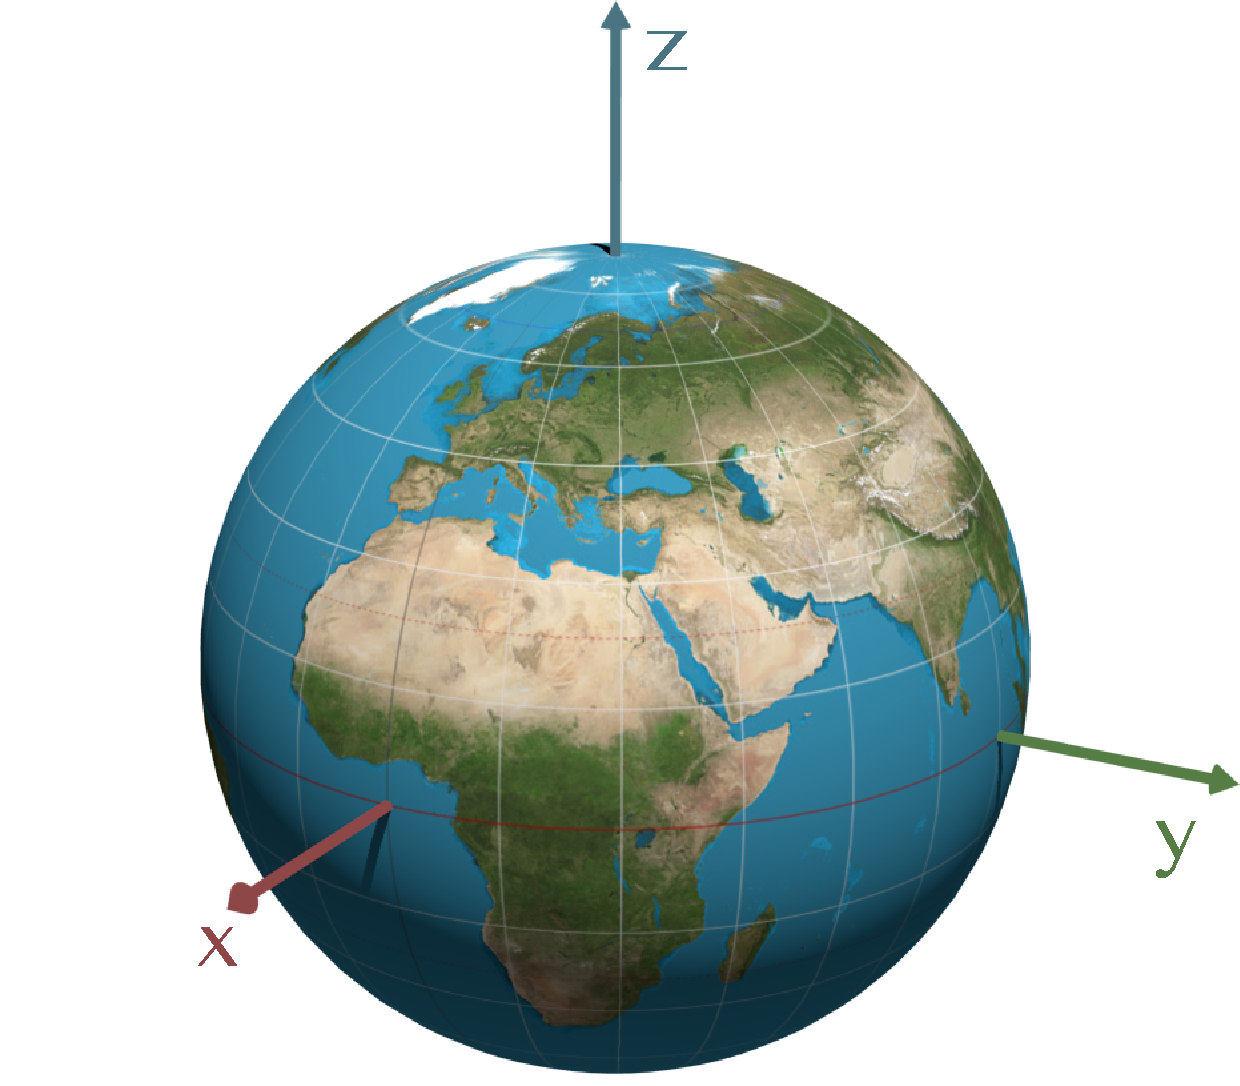
\includegraphics[scale=0.25]{figures/wgs84.pdf}
\caption{The WGS84 coordinate system and globe.}
\end{figure}